\documentclass[11pt]{aastex}
\usepackage{geometry}                % See geometry.pdf to learn the layout options. There are lots.
\geometry{letterpaper}                   % ... or a4paper or a5paper or ... 
%\geometry{landscape}                % Activate for for rotated page geometry
%\usepackage[parfill]{parskip}    % Activate to begin paragraphs with an empty line rather than an indent
\usepackage{graphicx}
\usepackage{amssymb}
\usepackage{epstopdf}
\DeclareGraphicsRule{.tif}{png}{.png}{`convert #1 `dirname #1`/`basename #1 .tif`.png}

\title{A Relation between Mass and Radius for 59 Exoplanets with $\rpl <  \rspecial$}
\author{L. M. Weiss \& G. W. Marcy}
%\date{}                                           % Activate to display a given date or no date

%---------------------------- Physical Quantities ------------------------------------%
\newcommand{\kms}{\ensuremath{\rm km\,s^{-1}}}
\newcommand{\ms}{\ensuremath{\rm m\,s^{-1}}}
\newcommand{\mse}{\ensuremath{\rm m\,s^{-1}}}
\newcommand{\gcmc}{\ensuremath{\rm g\,cm^{-3}}}
\newcommand{\gcc}{\gcmc}
\newcommand{\fluxunit}{\ensuremath{\rm erg\,s^{-1}\,cm^{-2}}}
\newcommand{\rhk}{\ensuremath{R^{\prime}_{\rm HK}}}	% Activity index R'_HK
\newcommand{\logrhk}{\ensuremath{\log\rhk}}		% log of R'_HK

\newcommand{\teff}{\ensuremath{T_{\rm eff}}}
\newcommand{\logg}{\ensuremath{\log{g}}}
\newcommand{\vsini}{\ensuremath{v \sin{i}}}
\newcommand{\feh}{[Fe/H]}
\newcommand{\logl}{\ensuremath{\log{L}}}

\newcommand{\rsun}{\ensuremath{R_\sun}}
\newcommand{\msun}{\ensuremath{M_\sun}}
\newcommand{\lsun}{\ensuremath{L_\sun}}

\newcommand{\rstar}{\ensuremath{R_\star}}
\newcommand{\mstar}{\ensuremath{M_\star}}
\newcommand{\loggstar}{\ensuremath{\logg_\star}}
\newcommand{\lstar}{\ensuremath{L_\star}}
\newcommand{\astar}{\ensuremath{a_\star}}
\newcommand{\loglstar}{\ensuremath{\log{L_\star}}}
\newcommand{\rhostar}{\ensuremath{\rho_\star}}

\newcommand{\rpl}{\ensuremath{R_{\rm P}}}
\newcommand{\mpl}{\ensuremath{M_{\rm P}}}
\newcommand{\lpl}{\ensuremath{L_{\rm P}}}
\newcommand{\rhopl}{\ensuremath{\rho_{\rm P}}}
\newcommand{\loggpl}{\ensuremath{\logg_{\rm P}}}
\newcommand{\teq}{\ensuremath{T_{\rm eq}}}

\newcommand{\rjup}{\ensuremath{R_{\rm J}}}
\newcommand{\mjup}{\ensuremath{M_{\rm J}}}
\newcommand{\rhojup}{\ensuremath{\rho_{\rm J}}}
\newcommand{\rearth}{\ensuremath{R_\earth}}
\newcommand{\mearth}{\ensuremath{M_\earth}}
\newcommand{\fearth}{\ensuremath{F_\earth}}

\newcommand{\msini}{\ensuremath{m \sin{i}}}
\newcommand{\mplsini}{\ensuremath{\mpl\sin{i}}}

\newcommand{\npl}{226~} % The number of exoplanets used to determine the MRF relation
\newcommand{\nhires}{42~} % The number of transiting planets in the HIRES paper
\newcommand{\nlm}{59~}
\newcommand{\rspecial}{4 \rearth}
\newcommand{\chisquared}{3.4~}
\newcommand{\chiquad}{6.5~}
\newcommand{\rms}{3.8 \mearth}

\begin{document}
\maketitle
%\begin{abstract}
We study the masses and radii of the 59 known exoplanets that have radii smaller than 4\rearth.  We find a linear relation of the form $\mpl/\mearth \approx 3\rpl$/\rearth.  The RMS of planet masses is \rms, and our best fit has reduced $\chi^2=\chisquared$, indicating a large diversity in planet compositions below 4\rearth.   \citet{WL2013} also find $\mpl \approx 3\rpl$ in 22 pairs of planets exhibiting transit timing variations, of which only 10 planets overlap with our sample.  The linear mass-radius relation translates to a decrease in planet density with increasing radius ($\mpl \propto \rhopl^{-2}$).  We find that exoplanets have densities of 5.5 \gcc\ at 2\rearth; exoplanets between 1-2\rearth\ are denser than Earth, indicating likely rocky compositions, whereas exoplanets between 2-4\rearth\ are less dense than Earth, indicating a significant fraction of H/He or water in their compositions. \citet{WL2013} note that the linear scaling between planet mass and radius is consistent with a constant escape velocity.  It is likely that photo-evaporation of the atmospheres of small planets near their stars sculpts the mass-radius relation for small planets at small orbital distances.
%\end{abstract}

\section{Introduction}
%\subsection{}

The Kepler Mission has found an abundance of planets with  $R < 4\rearth$ \citep{Batalha2013}.  However, in many systems, it is difficult to measure the masses of such small planets because the gravitational acceleration these planets induce on their host stars or neighboring planets is too small to detect with current telescopes and instruments.  How can we determine the composition of these planets?

Many scientists have explored the relation between planet mass and radius in the Solar system and beyond as a means for understanding exoplanet compositions\citep{Lissauer2011, Enoch2012, Kane2012, Seager2007}.  \citet{Weiss2013} have shown that for planets between a few and 150 of Earth masses, we can predict the radius of a planet from its mass and incident stellar flux.  However, below $\sim$4\rearth, the large apparent scatter in planet mass impedes accurate predictions of planet mass.  At 2\rearth, planets are observed to span a decade in density, from less dense than water to densities suggesting a solid iron composition.

One way to probe the scatter in planet mass is to attempt to measure the masses of more small planets.  Although uncertainties in the mass measurements for individual planets might be of order the planet mass, observing many small planets allows us to study the statistical distribution of planet masses for small planets.  \citet{Marcy2013} measured the masses of 42 small, transiting planets.  The planets were selected for their small size, and not based on predictions of their masses.  Therefore, these 42 new transiting planets offer an unbiased survey of the masses of small planets.  In this paper, we examine the relation between exoplanet mass and radius for the 40 exoplanets smaller than 4\rearth\ from \citet{Marcy2013}, plus 19 exoplanets smaller than 4\rearth\ from the literature, for a total of 59 exoplanets.  We also investigate how other parameters, including incident flux, orbital period, and stellar mass and radius, might correlate with the physical properties of these small exoplanets.

\section{Using Negative Planet Masses for Statistical Soundness}
\citet{Marcy2013} allow ``negative" planet masses as Keplerian orbital solutions to avoid a bias toward larger planet masses.  The typical uncertainty in RVs of a few meters per second that results from activity on the photosphere of the star is the same size or larger than the expected RV semi-amplitude induced by the planet's orbit.  Although there is no physical reason that the photospheric variability should phase with the orbit of a planet, occasionally the RVs appear to do so, in cases where there are only 10s of RVs of a star.  Fifty percent of the time, the RVs are correlated with the expected planet signature (i.e. the RVs are high when they should be high, and low when they should be low), and the other fifty percent of the time the RVs are anti-correlated with the expected planet signature (low when they should be high, and high when they should be low).  Because RVs from stellar activity that correlate with the expected planet signal will result in an over-estimate of planet mass, we must also include the RVs that are anti-correlated with the expected planet signal.  The use of a negative semi-amplitude for the RVs results in a ``negative" planet mass.  

Although no transiting planet really has a negative mass, the inclusion of these artificial negative planet masses allows us to treat the population of small planets statistically.  Since there is no bias toward large or small planet masses in our sample, we can take the weighted mean mass of planets of a given radius and get a value representative of the planet population.  If we did not include the negative masses, the weighted mean mass at a given radius would be too high.

\section{Justification for a Mass-Radius Relation for Small Exoplanets}
In Figure \ref{fig:rbin}, we show the weighted mean exoplanet mass in bins of width 1 \rearth.  On average, exoplanet mass increases with increasing radius, indicating an underlying correlation in the individual exoplanet masses and radii.  The individual measurements of planet mass and radius are shown in Figure \ref{fig:rm_4} and listed in Table \ref{tab:mrf}.

We calculate the probability that mass and radius are uncorrelated for planets smaller than 4\rearth.  First, we calculate the correlation coefficient (Pearson R test) $r=0.61$ .  There are 59 planets smaller than 4 \rearth, leaving 57 degrees of freedom, so the Student t value is 5.75.  The probability that these data are uncorrelated is $1.3 \times 10^{-6}$.  Thus, the masses and radii of planets between the sizes of Earth and Neptune are correlated.

\section{The Updated Mass-Radius Relation for Small Exoplanets}
The individual masses and radii shown in Figure \ref{fig:rm_4} suggest that exoplanet masses can be fit with a line.  We verify this with a traditional power-law fit and obtain $\mpl \propto \rpl$ as the best result.

The best linear fit to the data for $\rpl < \rspecial$ is:
$$
\mpl/\mearth = 0.2  +     2.6~\rpl/\rearth
$$
There are 59 exoplanets in this sample.  The reduced $\chi^2=\chisquared$, and the RMS $=\rms$.

To illustrate how this population of exoplanets compares to our Solar System, we plot the Solar System planets in Figure \ref{fig:rm_4} as blue triangles.  A quadratic fit to the exoplanet population happens to line up with the Solar System planets, but has a reduced $\chi^2$ that is twice as large as the linear fit to the exoplanets.  Since most of the exoplanets in this sample have $P < 50$ days, we do not expect them to behave the same way as Uranus and Neptune, which have orbital periods of tens of thousands of days.  Therefore, the hefty masses of Uranus and Neptune compared to planets of similar size that are closer to their stars is not unreasonable.  In fact, the difference in mass between Uranus and Neptune compared to closer-in planets of 4 \rearth\ distinguishes the quadratic fit as good for the solar system, as compared to the linear fit that is good for exoplanets.

\section{Discussion}
	
\subsection{Interpretation of the Mass-Radius Relation}
The correlation between exoplanet mass and radius for $\rpl < 4 \rearth$ indicates that Earth-size planets are less massive than Neptune-size planets.

The large reduced $\chi^2$ values for the linear and quadratic mass-radius relations indicate that these relations are not sufficient models to explain the variation in planet mass at a given radius.  Either a diversity of planet compositions, or correlation between the residuals and some other parameter, is required to explain the large scatter in planet mass.

The data are better described by a linear fit than a quadratic or cubic fit.  Since a cubic fit of $\mpl \propto \rpl^3$ describes how mass and radius relate for constant density, a fit of $\mpl \propto \rpl$ indicates that planet density decreases strongly as mass or radius increases (see Figure \ref{fig:rbin} and \ref{fig:rhor}).  This can be attributed to an increasing fraction of volatiles with increasing planet mass.

Previous work, including \citet{Lissauer2011} and \citet{Weiss2013}, suggest that the mass-radius relation is more like $\mpl \propto \rpl^2$ for small exoplanets.  However, these studies include Saturn or Saturn-like planets at the high-mass end of their populations.  Such planets are better described as part of the giant planet population.  Excluding Saturn-like planets gives a linear mass-radius relation for small planets, indicating that Saturn-like planets should not be used in the empirical study of the mass-radius relation for small planets.

In a study of planets with $\mpl < \sim20\mearth$, \citet{WL2013} found $\mpl/\mearth \approx 3 \rpl/\rearth$ in a sample of 22 pairs of planets that exhibited strong anti-correlated transit timing variations (TTVs).  Our independent assessment of 59 planets, 49 of which are not analyzed in \citet{WL2013}, agrees with this result.

\citet{WL2013} noted that a linear relation between planet mass and radius is dimensionally consistent with a constant escape velocity from the planet (i.e. $v_{\mathrm{esc}}^2 \sim \mpl/\rpl$).  While this is one interpretation of the linear mass-radius relation for small exoplanets, there are perhaps other valid physical interpretations.  For instance, a constant $\mpl/\rpl$ implies that the gravitational potential energy $U \propto \mpl/\rpl$ of exoplanets is constant.  This could be due to atmospheric particles escaping, but perhaps some other physical mechanism sets this energy level for exoplanets.

\subsection{Interpretation of Planet Compositions}
For detailed models of the compositions of the 42 new transiting planets presented in \citet{Marcy2013} and analyzed here, see \citet{Rogers2013}.  Here, we consider the statistical properties of planet densities.

The densities of exoplanets with $\rpl < \rspecial$ are shown in Figure \ref{fig:rhor}, and the densities binned by 1 \rearth\ are shown in Figure \ref{fig:rbin}.  Although the individual measurements of density for planets with $\rpl < 2 \rearth$ have large uncertainties (Figure \ref{fig:rhor}), the weighted mean densities (Figure \ref{fig:rbin}) for 0-1 \rearth\ and 1-2 \rearth\ show the continuation of the trend that smaller planets have higher densities.  Figure \ref{fig:rhor} shows a dashed line at the density of Earth.  Planets smaller than 2 \rearth\ tend to be denser than Earth, whereas planets larger than 2 \rearth\ tend to be less dense than Earth.  However, since rock and other materials are compressible, planets that are as dense as Earth but have larger radii are not necessarily solid rock; they need some lighter materials, such as water or a H/He envelope, to achieve the density of Earth.

\subsection{The Possible Role of Photoevaporation in Sculpting Small Planets}
Strong stellar irradiation can either inflate a planet, as with hot Jupiters \citep{Seager2007}, or it can photoionize and strip the planet's atmosphere, leaving a dense core \citep{Lopez2012}.  Possible evidence for these processes can be seen in Figure \ref{fig:flux_radius}, which shows that for massive planets ($\mpl > 60 \mearth $ or $\rpl > \rspecial$), high incident flux correlates with larger radius, whereas for low-mass planets ($\mpl < 60 \mearth $ or $\rpl < \rspecial$), high incident flux correlates with smaller radius.

Another way to describe how incident flux relates to exoplanet size is that for low levels of incident stellar flux (less than 100 times what Earth receives), planets range in size from Earth to Jupiter.  However, at higher incident flux, there are only hot Earths (which might have been photo-evaporated) and hot Jupiters (which have been inflated).  In other words, there are no hot Neptunes.  Given the detection of hot and cold Earths, hot and cold Jupiters, and cold Neptunes, it seems unlikely that a detection bias causes the dearth of hot Neptunes; rather, their absence is likely astrophysical.

\begin{comment}
How significant is the decrease in planet size with increasing planet flux for small exoplanets?  For $\rpl < \rspecial$, we find a correlation Pearson R coefficient between planet radius and incident stellar flux of $r=-0.19$.  Over a sample of 71 planets, this corresponds to a Student-t value of $t=-1.6$, indicating a probability of 0.11 that these variables are uncorrelated.  Repeating this calculation for a larger sample of exoplanets (for instance, the entire catalog of Kepler planets candidates, for which \rpl and the incident flux on the planet are known) would reveal whether this correlation is real.
\end{comment}

\subsection{A Correlation between Planet Mass and Stellar Metallicity for Small Planets}
The stellar metallicities of the stars in our sample are determined by spectroscopy and/or asteroseismology, yielding values accurate to 0.1 dex.  We find a correlation between planet mass and stellar metallicity for planets smaller than 4\rearth.  The Pearson R-value of the correlation is 0.32, resulting in a probability of 2\% that planet mass and stellar metallicity are not correlated.  In other words, we find a correlation between planet mass and metallicity with $2\sigma$ confidence in exoplanets smaller than 4\rearth.  In Figure \ref{fig:m_fe}, we plot planet mass and planet radius against stellar metallicity for the planets in our sample.

\citet{Buchhave2012} note that planets smaller than 4\rearth\ form around stars with a large range of metallicities.  Their study includes 226 Kepler exoplanet candidates smaller than 4\rearth, for which they obtained spectroscopic measurements of [m/H] in the host stars.  Our work uses [Fe/H] as a metallicity indicator, and we are only considering validated exoplanets.  Although \citet{Buchhave2012} find no relation between exoplanet occurrence and host star metallicity for $\rpl < 4\rearth$, they do not comment on the relation between exoplanet size and host star metallicity for small planets.  Therefore, our finding that planet mass correlates with stellar metallicity for $\rpl < 4\rearth$ does not contradict their result.

\subsection{Absence of Correlations with Mass Residuals}
We examine the possibility that the residuals to the mass-radius relation correlate with some other parameters.  We consider how the residual mass (exoplanet mass minus predicted mass) correlates with the incident flux from the star, the semi-major axis, the orbital period, the stellar mass, and the stellar radius.  The residual mass did not correlate with any of these properties; the highest Pearson-R coefficient was $0.1$.  For all of the parameters listed above, the probability that the mass residuals do not correlate with each parameter is at least 30\% (i.e. the probability that the mass residuals correlate with any of the above parameters is at most 70\%).  While we cannot rule out correlation between the mass residuals and other orbital and physical properties, we do not find evidence for any correlation to the residuals.

\section{Conclusions}
For exoplanets with $\rpl < \rspecial$ and $P < ~\sim100$ days, planet radius correlates with planet mass with linear scaling: $\mpl/\mearth \approx 3\rpl/\rearth$, indicating that larger planets have substantially more volatiles than smaller planets.  This relation is also different than what we observe for the Solar System planets smaller than Saturn: $\mpl \propto \rpl^2$.  Uranus and Neptune are more massive than the exoplanets of their size in this sample, and they are also at much larger orbital distances than any of the exoplanets in our sample.  A study of exoplanets of 3-4 \rearth with orbital periods of dozens of years would better contextualize the mass and radius of Uranus and Neptune.

One reason Uranus and Neptune might be more massive than closer-in planets of the same size is that incident stellar flux might photo evaporate the atmospheres of closer-in counterparts, causing mass loss.  The correlations between planet size and incident flux from the star for both large and small planets, and the absence of hot Neptunes, indicate that incident stellar flux of more than 100 times what Earth receives might play a key role in sculpting close-in planets.

%% The values (usually only l,r and c) in the last part of
%% \begin{deluxetable}{} command tell LaTeX how many columns
%% there are and how to align them.
\begin{deluxetable}{lllllll}

%% Keep a portrait orientation


%% Over-ride the default font size
%% Use 10pt
\tabletypesize{\tiny}

\tablewidth{0pt} %to over-ride the default table width.
%% If you are unhappy with the default look at the end of the
%% *.log file to see what the default was set at before adjusting
%% this value.

%% This is the title of the table.
\tablecaption{Exoplanets with Mass Upper Limits and $\rpl < \rspecial$}
%% This command over-rides LaTeX's natural table count
%% and replaces it with this number.  LaTeX will increment 
%% all other tables after this table based on this number
\tablenum{1}
\label{tab:mrf}

%% The \tablehead gives provides the column headers.  It
%% is currently set up so that the column labels are on the
%% top line and the units surrounded by ()s are in the 
%% bottom line.  You may add more header information by writing
%% another line between these lines. For each column that requries
%% extra information be sure to include a \colhead{text} command
%% and remember to end any extra lines with \\ and include the 
%% correct number of &s.
\tablehead{\colhead{Name} & \colhead{Per} & \colhead{Mass} & \colhead{Radius} & \colhead{Flux} & \colhead{First Ref.} & \colhead{Orbit Ref.} \\ 
\colhead{} & \colhead{(d)} & \colhead{($\mearth$)} & \colhead{($\rearth$)} & \colhead{($\fearth$)} & \colhead{} & \colhead{} } 

%% All data must appear between the \startdata and \enddata commands
\startdata
            55 Cnc e &      0.737 &       8.38$\pm$0.39       &       2.21$\pm$0.15       &   2439.690 &                     \citet{McArthur2004} &                         \citet{Endl2012}\\ 
           CoRoT-7 b &      0.854 &       5.02$\pm$0.86       &       1.68$\pm$0.09       &   1779.433 &             \citet{Queloz2009,Leger2009} &                       \citet{Queloz2009}\\ 
           GJ 1214 b &      1.580 &       6.26$\pm$0.91       &       2.80$\pm$0.24       &     16.631 &                  \citet{Charbonneau2009} &                       \citet{Carter2011}\\ 
          HD 97658 b &      9.491 &       7.87$\pm$0.73       &       2.34$\pm$0.16       &     48.106 &                       \citet{Howard2011} &                     \citet{Dragomir2013}\\ 
         Kepler-10 b &      0.837 &       4.54$\pm$1.25       &       1.42$\pm$0.03       &   3572.048 &                      \citet{Batalha2011} &                      \citet{Batalha2011}\\ 
         Kepler-11 b &     10.304 &       1.90$\pm$1.20       &       1.80$\pm$0.04       &    126.512 &                     \citet{Lissauer2011} &                     \citet{Lissauer2013}\\ 
         Kepler-11 c &     13.024 &       2.90$\pm$2.20       &       2.87$\pm$0.06       &     91.443 &                     \citet{Lissauer2011} &                     \citet{Lissauer2013}\\ 
         Kepler-11 d &     22.684 &       7.30$\pm$1.10       &       3.12$\pm$0.07       &     43.563 &                     \citet{Lissauer2011} &                     \citet{Lissauer2013}\\ 
         Kepler-11 f &     46.689 &       2.00$\pm$0.80       &       2.49$\pm$0.06       &     16.747 &                     \citet{Lissauer2011} &                     \citet{Lissauer2013}\\ 
         Kepler-18 b &      3.505 &       6.90$\pm$3.48       &       2.00$\pm$0.10       &    462.244 &                      \citet{Borucki2011} &                      \citet{Cochran2011}\\ 
         Kepler-20 b &      3.696 &       8.47$\pm$2.12       &       1.91$\pm$0.16       &    346.711 &                      \citet{Borucki2011} &                      \citet{Gautier2012}\\ 
         Kepler-20 c &     10.854 &      15.73$\pm$3.31       &       3.07$\pm$0.25       &     82.445 &                      \citet{Borucki2011} &                      \citet{Gautier2012}\\ 
         Kepler-20 d &     77.612 &       7.53$\pm$7.22       &       2.75$\pm$0.23       &      5.985 &                      \citet{Borucki2011} &                      \citet{Gautier2012}\\ 
         Kepler-36 b &     13.840 &       4.46$\pm$0.30       &       1.48$\pm$0.03       &    217.365 &                      \citet{Borucki2011} &                       \citet{Carter2012}\\ 
         Kepler-36 c &     16.239 &       8.10$\pm$0.53       &       3.68$\pm$0.05       &    175.646 &                       \citet{Carter2012} &                       \citet{Carter2012}\\ 
         Kepler-68 b &      5.399 &       8.30$\pm$2.30       &       2.31$\pm$0.03       &    409.092 &                      \citet{Borucki2011} &                    \citet{Gilliland2013}\\ 
         Kepler-68 c &      9.605 &       4.38$\pm$2.80       &       0.95$\pm$0.04       &    189.764 &                      \citet{Batalha2013} &                    \citet{Gilliland2013}\\ 
           Kepler-78 b &      0.354 &       1.78$\pm$0.30       &       1.20$\pm$0.09       &   3093.388 &              \citet{Sanchis-Ojeda2013} &              Howard et al. (2013, submitted)\\ 
            KOI-94 b &      3.743 &       9.40$\pm$4.50       &       1.77$\pm$0.17       &   1155.374 &                        \citet{Batalha2013} &                        \citet{Weiss2013}\\ 
           KOI-41.01 &     12.816 &       0.85$\pm$4.00       &       2.20$\pm$0.05       &    213.371 &                      \citet{Borucki2011} &                        \citet{Marcy2013}\\ 
           KOI-41.02 &      6.887 &       7.34$\pm$3.20       &       1.32$\pm$0.04       &    472.831 &                      \citet{Borucki2011} &                        \citet{Marcy2013}\\ 
           KOI-41.03 &     35.333 &      -4.36$\pm$4.10       &       1.61$\pm$0.05       &     55.812 &                      \citet{Borucki2011} &                        \citet{Marcy2013}\\ 
           KOI-69.01 &      4.727 &       2.59$\pm$2.00       &       1.50$\pm$0.03       &    220.120 &                      \citet{Borucki2011} &                        \citet{Marcy2013}\\ 
           KOI-82.01 &     16.146 &       8.93$\pm$2.00       &       2.22$\pm$0.07       &     17.278 &                      \citet{Borucki2011} &                        \citet{Marcy2013}\\ 
           KOI-82.02 &     10.312 &       3.80$\pm$1.80       &       1.18$\pm$0.04       &     31.184 &                      \citet{Borucki2011} &                        \citet{Marcy2013}\\ 
           KOI-82.03 &     27.454 &       0.62$\pm$3.30       &       0.88$\pm$0.03       &      8.250 &                      \citet{Borucki2011} &                        \citet{Marcy2013}\\ 
           KOI-82.04 &      7.071 &      -1.58$\pm$2.00       &       0.58$\pm$0.02       &     51.315 &                      \citet{Borucki2011} &                        \citet{Marcy2013}\\ 
           KOI-82.05 &      5.287 &       0.41$\pm$1.60       &       0.47$\pm$0.02       &     78.407 &                      \citet{Borucki2011} &                        \citet{Marcy2013}\\ 
          KOI-104.01 &      2.508 &      10.84$\pm$1.40       &       3.51$\pm$0.15       &    214.674 &                      \citet{Borucki2011} &                        \citet{Marcy2013}\\ 
          KOI-108.01 &     15.965 &      14.11$\pm$4.70       &       3.37$\pm$0.09       &    124.197 &                      \citet{Borucki2011} &                        \citet{Marcy2013}\\ 
          KOI-116.01 &     13.571 &      10.44$\pm$3.20       &       2.50$\pm$0.32       &     84.462 &                      \citet{Borucki2011} &                        \citet{Marcy2013}\\ 
          KOI-116.02 &     43.844 &      11.17$\pm$5.80       &       2.56$\pm$0.33       &     15.645 &                      \citet{Borucki2011} &                        \citet{Marcy2013}\\ 
          KOI-116.03 &      6.165 &       0.15$\pm$2.80       &       0.82$\pm$0.11       &    239.077 &                      \citet{Borucki2011} &                        \citet{Marcy2013}\\ 
          KOI-116.04 &     23.980 &      -6.39$\pm$7.00       &       0.95$\pm$0.13       &     43.146 &                      \citet{Borucki2011} &                        \citet{Marcy2013}\\ 
          KOI-122.01 &     11.523 &      13.00$\pm$2.90       &       3.42$\pm$0.09       &    182.708 &                      \citet{Borucki2011} &                        \citet{Marcy2013}\\ 
          KOI-123.01 &      6.482 &       1.30$\pm$5.40       &       2.37$\pm$0.07       &    444.879 &                      \citet{Borucki2011} &                        \citet{Marcy2013}\\ 
          KOI-123.02 &     21.223 &       2.22$\pm$7.80       &       2.52$\pm$0.07       &     94.934 &                      \citet{Borucki2011} &                        \citet{Marcy2013}\\ 
          KOI-148.01 &      4.778 &       3.94$\pm$2.10       &       1.88$\pm$0.10       &    168.932 &                      \citet{Borucki2011} &                        \citet{Marcy2013}\\ 
          KOI-148.02 &      9.674 &      14.61$\pm$2.30       &       2.71$\pm$0.14       &    225.109 &                      \citet{Borucki2011} &                        \citet{Marcy2013}\\ 
          KOI-148.03 &     42.896 &       7.93$\pm$4.60       &       2.04$\pm$0.11       &     13.545 &                      \citet{Borucki2011} &                        \citet{Marcy2013}\\ 
          KOI-153.01 &      8.925 &      -4.60$\pm$6.20       &       2.19$\pm$0.06       &     50.981 &                      \citet{Borucki2011} &                        \citet{Marcy2013}\\ 
          KOI-153.02 &      4.754 &       7.10$\pm$3.30       &       1.82$\pm$0.05       &     63.986 &                      \citet{Borucki2011} &                        \citet{Marcy2013}\\ 
          KOI-244.02 &      6.239 &       9.60$\pm$4.20       &       2.71$\pm$0.05       &    667.269 &                      \citet{Borucki2011} &                        \citet{Marcy2013}\\ 
          KOI-245.01 &     39.792 &       1.87$\pm$9.08       &       1.94$\pm$0.06       &      7.710 &                      \citet{Borucki2011} &                        \citet{Marcy2013}\\ 
          KOI-245.02 &     21.302 &       3.35$\pm$4.00       &       0.75$\pm$0.03       &     16.291 &                      \citet{Borucki2011} &                        \citet{Marcy2013}\\ 
          KOI-245.03 &     13.367 &       2.78$\pm$3.70       &       0.32$\pm$0.02       &     37.373 &                      \citet{Borucki2011} &                        \citet{Marcy2013}\\ 
          KOI-246.01 &      5.399 &       5.97$\pm$1.70       &       2.33$\pm$0.02       &    375.530 &                      \citet{Borucki2011} &                        \citet{Marcy2013}\\ 
          KOI-246.02 &      9.605 &       2.18$\pm$3.50       &       1.00$\pm$0.02       &    220.199 &                      \citet{Borucki2011} &                        \citet{Marcy2013}\\ 
          KOI-261.01 &     16.238 &       8.46$\pm$3.40       &       2.67$\pm$0.22       &     73.950 &                      \citet{Borucki2011} &                        \citet{Marcy2013}\\ 
          KOI-283.01 &     16.092 &      16.13$\pm$3.50       &       2.41$\pm$0.20       &     71.656 &                      \citet{Borucki2011} &                        \citet{Marcy2013}\\ 
          KOI-283.02 &     25.517 &       8.25$\pm$5.90       &       0.84$\pm$0.07       &     28.891 &                      \citet{Borucki2011} &                        \citet{Marcy2013}\\ 
          KOI-292.01 &      2.587 &       3.51$\pm$1.90       &       1.48$\pm$0.13       &    851.551 &                      \citet{Borucki2011} &                        \citet{Marcy2013}\\ 
          KOI-299.01 &      1.542 &       3.55$\pm$1.60       &       1.99$\pm$0.22       &   1581.816 &                      \citet{Borucki2011} &                        \citet{Marcy2013}\\ 
          KOI-305.01 &      4.604 &       6.15$\pm$1.30       &       1.48$\pm$0.08       &     90.372 &                      \citet{Borucki2011} &                        \citet{Marcy2013}\\ 
          KOI-321.01 &      2.426 &       6.35$\pm$1.40       &       1.43$\pm$0.03       &    713.204 &                      \citet{Borucki2011} &                        \citet{Marcy2013}\\ 
          KOI-321.02 &      4.623 &       2.71$\pm$1.80       &       0.85$\pm$0.03       &    291.503 &                      \citet{Borucki2011} &                        \citet{Marcy2013}\\ 
         KOI-1442.01 &      0.669 &       0.06$\pm$1.20       &       1.07$\pm$0.02       &   3645.770 &                      \citet{Borucki2011} &                        \citet{Marcy2013}\\ 
         KOI-1612.01 &      2.465 &       0.48$\pm$3.20       &       0.82$\pm$0.03       &   1691.964 &                      \citet{Borucki2011} &                        \citet{Marcy2013}\\ 
         KOI-1925.01 &     68.958 &       2.69$\pm$6.20       &       1.19$\pm$0.03       &      6.165 &                      \citet{Borucki2011} &                        \citet{Marcy2013}\\ 
\enddata

%% Include any \tablenotetext{key}{text}, \tablerefs{ref list},
%% or \tablecomments{text} between the \enddata and 
%% \end{deluxetable} commands

%% No \tablecomments indicated

%% No \tablerefs indicated

\end{deluxetable}

\clearpage
\begin{figure}[htbp] %  figure placement: here, top, bottom, or page
   \centering
   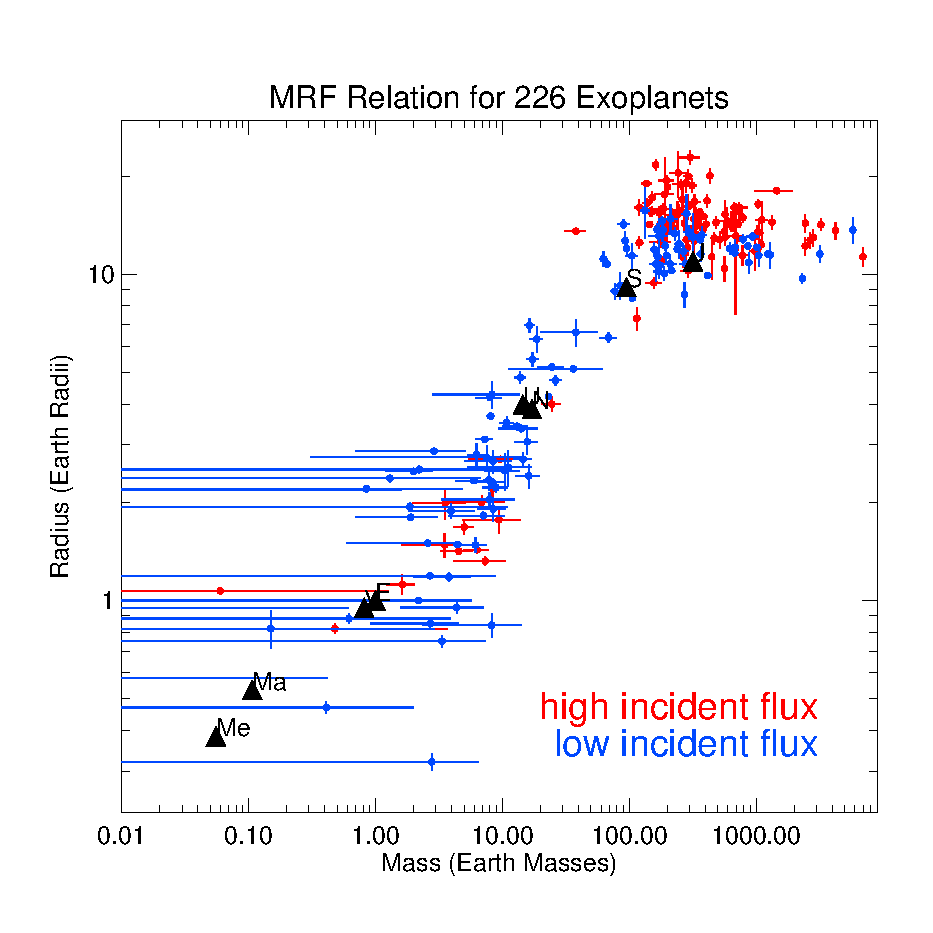
\includegraphics[width=6in]{mrf.eps} 
   \caption{Radius vs. mass for exoplanets with measured masses and radii.  Planets receiving lower than the median incident flux from this sample (459 times the incident flux at Earth) are blue; those receiving higher than the median incident flux are red.  The Solar System planets are over plotted as black triangles for comparison.  For giant planets ($\mpl \geq \frac{1}{2} M_{\mathrm{Sat}}$), planet radius correlates with incident flux, whereas for the smaller planets, radius and incident flux appear anti-correlated (see Figure \ref{fig:flux_radius}).}
   \label{fig:mrf}
\end{figure}

\begin{figure}[htbp] %  figure placement: here, top, bottom, or page
   \centering
    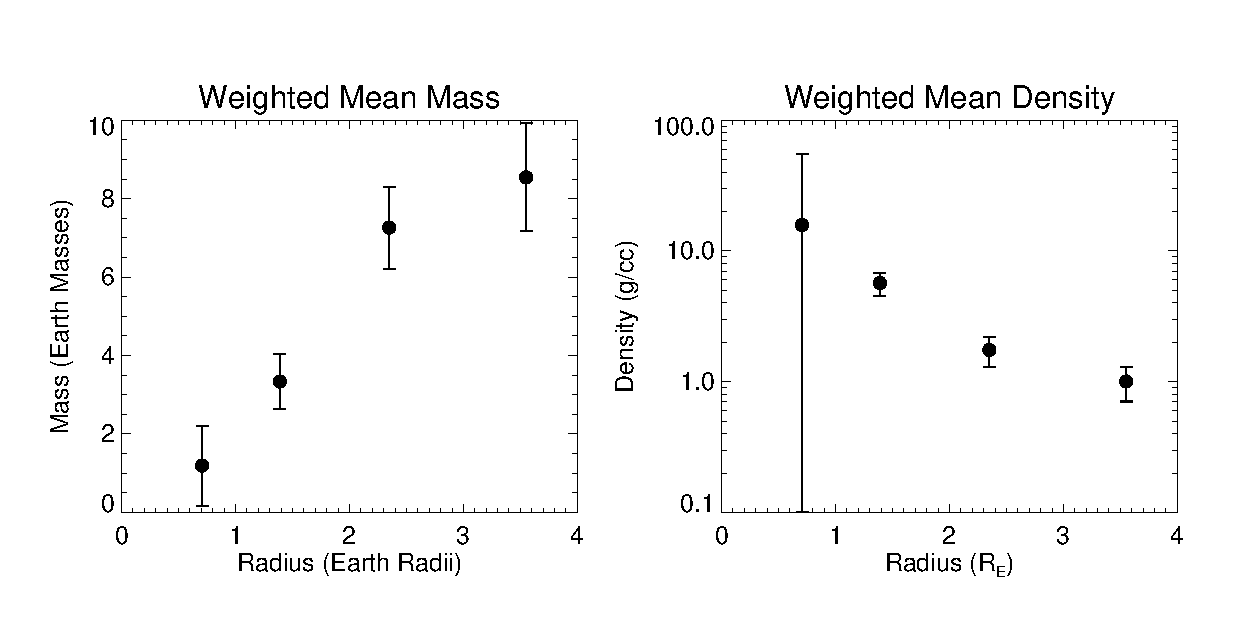
\includegraphics[width=6in]{mr_bin.eps} 
   \caption{The weighted mean mass (left) and density (right) for exoplanets with $\rpl < \rspecial$ in bins of 1 \rearth.  The error bars are the weighted uncertainties in the means.  Larger exoplanet radii correlate with larger masses but lower densities, indicating that large planets have a larger mass fraction of volatiles than small planets.}
   \label{fig:rbin}
\end{figure}

\begin{figure}[htbp] %  figure placement: here, top, bottom, or page
   \centering
    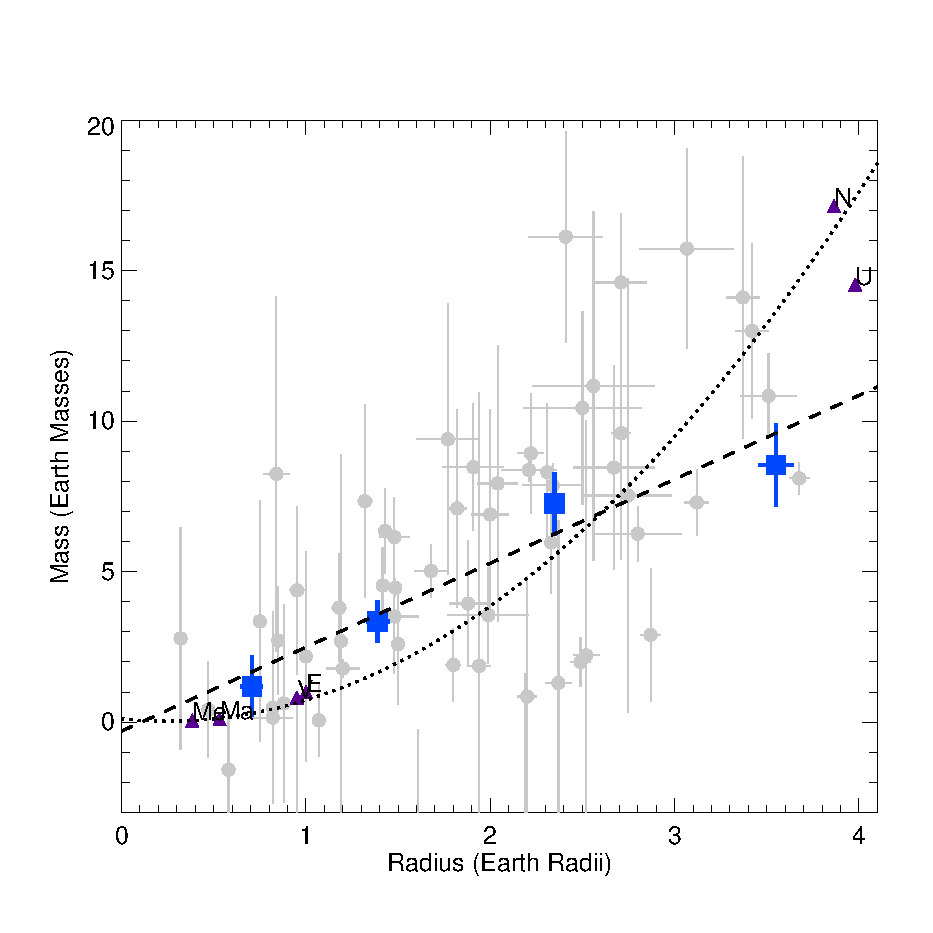
\includegraphics[width=6in]{rm_small4.eps} 
   \caption{\small Mass vs. radius for 59 planets with $\rpl < 4 \rearth$ and 1$\sigma$ uncertainties are plotted as gray dots.  Blue squares represent the weighted mean mass in bins of 1 \rearth with error bars representing the uncertainty in the mean mass (as in Figure \ref{fig:rbin}).  The blue square are to guide the eye only; they were not used in any of the fitting procedures.  The dashed line is the best linear fit to the 59 exoplanets: $\mpl/\mearth = 0.2 + 2.6 \times \rpl/\rearth$, $\chi^2/\nu = \chisquared$.  The solar system planets were excluded from the linear fit.  Note that a linear fit goes through the the weighted mean of the exoplanet population.  The dotted line is the best quadratic fit to the 59 exoplanets plus 6 Solar System planets: $\mpl = 0.1 - 0.6 \rpl + 1.25 \rpl^2$.  The solar system planets are plotted as purple triangles.  We assumed errors in \mpl and \rpl for S.S. planets were $10^{-5}$ of their values.   Note that Uranus and Neptune are much colder than the exoplanets in this sample.}
   \label{fig:rm_4}
\end{figure}

\begin{figure}[htbp] %  figure placement: here, top, bottom, or page
   \centering
    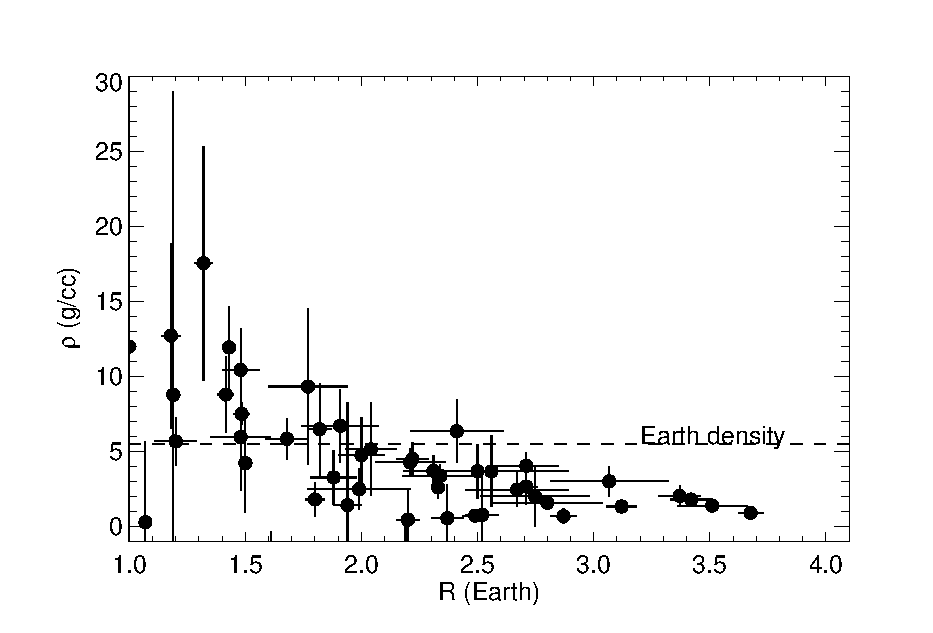
\includegraphics[width=6in]{rhor_4.eps} 
   \caption{Density vs. radius for planets with $\rpl < \rspecial $ and $1\sigma$ uncertainties.  Smaller planets are denser than larger planets.  For reference, the density of Earth (5.5 \gcc) is shown as a dashed line.  Planets smaller than 2\rearth\ are denser than Earth, indicating likely rocky compositions; planets larger than 2 \rearth\ are less dense than Earth, indicating moderate amounts of H/He or water in their compositions.  The monotonic decrease in density with increasing planet radius from 1-4 \rearth\ indicates a monotonically increasing fraction of volatiles.}
   \label{fig:rhor}
\end{figure}


\begin{figure}[htbp] %  figure placement: here, top, bottom, or page
   \centering
      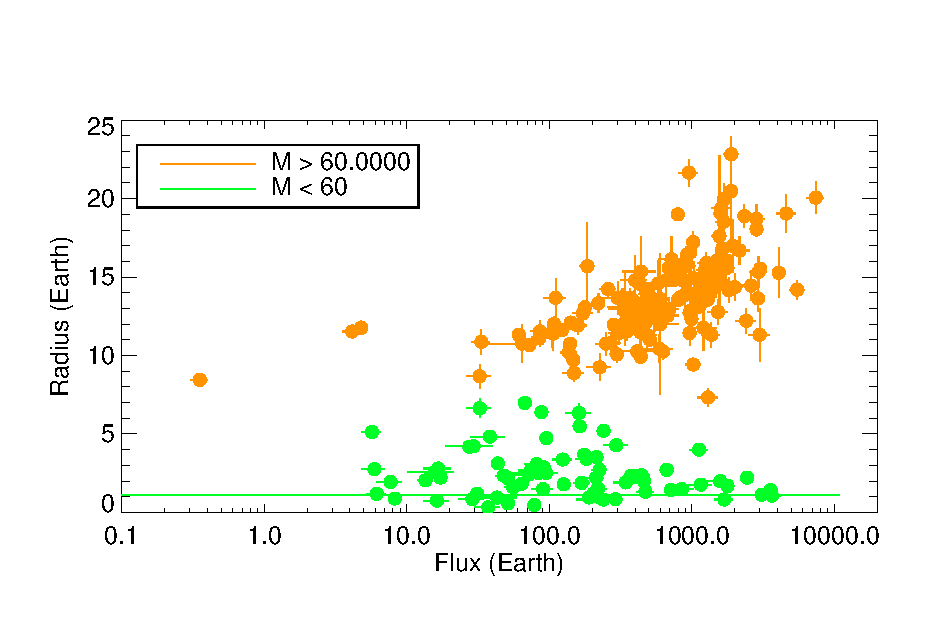
\includegraphics[width=6in]{flux_dependence.eps} 
   \caption{Radius vs. flux and $1\sigma$ uncertainties for exoplanets with measured masses and radii.  Giant planets are orange; low-mass planets are green.  For giant planets, radius increases with increasing incident flux from the star; for small planets, radius slightly decreases with increasing flux, especially above a few hundred Earth fluxes.  There are no hot Neptunes.  Note that all the planets with $\rpl < 4 \rearth$ are in the low-mass population.}
   \label{fig:flux_radius}
\end{figure}


\begin{figure}[htbp] %  figure placement: here, top, bottom, or page
   \centering
      \includegraphics[width=6in]{m_fe.png} 
   \caption{Planet mass vs. stellar metallicity (left) and planet radius vs. stellar metallicity (right), with $1\sigma$ errors.  The absence of points in the upper left and lower right corners of each plot indicates a weak correlation between planet mass (or radius) and stellar metallicity.  The Pearson R-value of the correlation is 0.32, and the probability that these parameters are uncorrelated is 2\%.}
\end{figure}


\begin{comment}
\begin{figure}[htbp] %  figure placement: here, top, bottom, or page
   \centering
    \includegraphics[width=6in]{mr_residuals.eps} 
   \caption{Mass residuals (measured minus predicted mass) vs. radius for planets with $\rpl  < \rspecial$ and 1$\sigma$ uncertainties.  The correlation between mass residuals and orbital parameters is too small to be significant.}
   \label{fig:resids}
\end{figure}
\end{comment}

%%%%%%%%%%%%% Discussion %%%%%%%%%%%%%%%%%%%%%%%%%%%%%%%%
\clearpage

\bibliography{exoplanet_papers}{}
\bibliographystyle{apj}

\end{document}  